% Niniejszy plik stanowi przyklad formatowania pracy magisterskiej na
% Wydziale MIM UW.  Szkielet uzytych polecen mozna wykorzystywac do
% woli, np. formatujac wlasna prace.
%
% Zawartosc merytoryczna stanowi oryginalnosiagniecie
% naukowosciowe Marcina Wolinskiego.  Wszelkie prawa zastrzezone.

% Copyright (c) 2001 by Marcin Wolinski <M.Wolinski@gust.org.pl>
% Poprawki spowodowane zmianami przepisów - Marcin Szczuka, 1.10.2004
% Poprawki spowodowane zmianami przepisow i ujednolicenie 
% - Seweryn Karlowicz, 05.05.2006
% Zmiany dla wersji angielskiej - Michal Derezinski, 10.05.2012
\documentclass{pracamgren}

\usepackage[utf8]{inputenc}
\usepackage[T1]{fontenc}
\usepackage[titletoc]{appendix}
\usepackage[backend=bibtex]{biblatex}
\usepackage{hyperref}
\bibliography{atari-ram.bib} 

\hypersetup{colorlinks=true}
\author{Jakub Sygnowski}

\nralbumu{319394}

\title{Learning agents to play Atari games using the RAM memory}

\tytul{Uczenie agentów grających w gry Atari na podstawie pamięci RAM}

\kierunek{Informatics}

% W wersji angielskiej, zakres ma byc po angielsku.
% \zakres{Tu wpisac, jesli trzeba, jedna z opcji podanych wyzej}

% Praca wykonana pod kierunkiem:
% (podac tytul/stopien imie i nazwisko opiekuna
% Instytut
% ew. Wydzial ew. Uczelnia (jezeli nie MIM UW))
% W wersji angielskiej, ma byc po angielsku.
\opiekun{dr hab. Henryk Michalewski\\
Institute of Mathematics\\
}

% miesiac i rok (po angielsku):
\date{November 2016}

%Podac dziedzine wg klasyfikacji Socrates-Erasmus:
\dziedzina{ 
%11.3 Informatyka\\ 
11.4 Sztuczna inteligencja\\ 
}

\dziedzinaang{
%11.3 Informatics, Computer Science\\ 
11.4 Artificial Intelligence\\ 
}

%Klasyfikacja tematyczna wedlug AMS (matematyka) lub ACM (informatyka)
\klasyfikacja{Metodologie Obliczeniowe\\
  Uczenie maszynowe\\
  Algorytmy uczenia maszynowego\\
  Programowanie dynamiczne w procesach decyzyjnych Markowa\\
  Q-learning
}

\klasyfikacjaang{Computing Methodologies\\
  Machine learning\\
  Machine learning algorithms\\
  Dynamic programming for Markov decision processes\\
  Q-learning
}

\keywords{Atari, deep Q-learning, pamięć RAM}

\keywordsang{Atari, deep Q-learning, RAM}

% Tu jest dobre miejsce na Twoje wlasne makra i~srodowiska:
\newtheorem{defi}{Definition}[section]

% koniec definicji

\begin{document}
\maketitle

\streszczenie{
  Niedawne ulepszenia w metodach treningu i powstanie nowych rodzajów sieci neuronowych doprowadziło do stworzenia nowych algorytmów uczenia ze wzmacnianiem. Popularnym zadaniem testującym możliwości tych algorytmów są gry Atari, symulowane na współczesnych komputerach. W naszej pracy adaptujemy popularny i skuteczny algorytm deep Q-learning, który w oryginalnej wersji używa konwolucyjnych sieci neuronowych do przypadku, gdzie wejściem nie jest ekran gry, ale stan pamięci RAM maszyny Atari. Prezentujemy implementację naszej metody i wyniki ewaluacji jej kilku wersji na wybranych grach Atari.
}

\begin{abstract}
  Recent advances in the methods of training and invention of the new kinds of neural networks led to creation of the new reinforcement learning algorithms. Popular framework for testing these algorithms are Atari games, simulated on modern computers. In our work we adapt a popular and efficient deep Q-learning algorithm, which in its original version uses convolutional neural networks, to the case when it is given not the game screen, but the RAM state of the Atari machine. We present implementation of our method and results of the evaluation of its few versions on the chosen Atari games.
\end{abstract}

\nocite{*}

\tableofcontents
%\listoffigures
%\listoftables

\chapter*{Introduction}
\addcontentsline{toc}{chapter}{Introduction}
From the very beginning of computing, humanity is vividly interested in simulating the thought process of a mind through the field of artificial intelligence. The advances in theoretical aspects of computer science, as well as methods of manufacturing faster computers made the speed of progress of AI methods ever increasing. One can see it in many domains---from self-driving cars, through machine translation, to speech synthesis. A particularly neat area for testing intelligent algorithms is playing games.

Games are often used as a benchmark of the possibilities of AI, because on one hand, they have a well-defined evaluation metric and are cheap to simulate (which is not the case e.g. with medical diagnosis or steering robots) and, on the other hand, they offer limitless variants and levels of difficulty. While some of them (like chess, Go) require from playing agents quick search and accurate state evaluation \cite{alphago}, others (e.g.~Doom) need reflex and good object recognition, and some (e.g. Morpion) enjoy theorem-proving methods and being treated with linear programming \cite{morpion}.

In this work, we focus on games published for the Atari 2600---a game console from the previous century. While these are a very small subset of all games\footnote{There are around 470~games produced for Atari}, their variability offers a group of challenges. In opposition to the current trend \cite{nips-dqn, nature-dqn, a3c}, we train agents to play the games, seeing the RAM input instead of the screen. This problem is scarcely considered in literature (we are aware only of a poorly performing RAM agent in \cite{ale}); most of the methods described here are based on our previous work \cite{our-paper}, presented on Computer Games Workshop during International Joint Conference in Artificial Intelligence $2016$ in New~York.

In this thesis, we make a couple of contributions toward making better RAM-based Atari playing agents. First, we review the foundations of the models we will be using in chapter \ref{foundations}. They contain both ground work on reinforcement learning from 80s and~the evolving since $2012$ methods of building and training neural networks.

Second, in chapter \ref{dqn}, we define Deep Q-learning---the algorithm we use to train playing agents.
Chapter \ref{dqn-ram} consists of modification to original Deep Q-learning we tried to make it work for RAM input.
In chapter \ref{extensions} we show and discuss the results of evaluation of the trained methods.
Chapter \ref{conclusions} contains ideas for further extending this work.
In appendix \ref{icm} we describe the technical difficulties we overcame to feasibly train the models on the GPU cluster of our University's Interdisciplinary Centre for Mathematical and Computational Modelling.
\section*{Acknowledgements}
\addcontentsline{toc}{section}{Acknowledgements}
First of all, I would like to thank my advisor, dr~hab. Henryk~Michalewski, for spending numerous hours to complete the project. He not only offered interesting scientific discussions, but also the help on the technical side.

I would also like to thank Marc G. Bellamare for suggesting the topic of the thesis and Deepsense.io for supporting our attendance at the IJCAI conference.

The computation performed within this project were carried out with the support of grant GG63-11 awarded by the Interdisciplinary Centre for Mathematical and Computational Modelling (ICM) University of Warsaw.


\chapter{Foundations}\label{foundations}
Most of the groundwork of the methods we will be using was invented in the second half of the 20th century. They include reinforcement learning---a general framework defining the aim of the playing algorithm, Q-learning---a simple algorithm to learn to play a game, and basics of neural networks---the statistical model that was used to overcome Q-learning's limitations.
This foundation work, joined with the recent (after $2010$) advances in the methods of training and architectures of neural networks allowed to vastly improve the former results.

This chapter discusses these methods, as well as describes the Atari machine, as the games we are interested in playing are created for this platform.

\section{Reinforcement learning}
To create an algorithm learning to play a game or solve any other problem, we first have to formally define what the problem is. We will model Atari games within the framework called reinforcement learning. The main property distinguishing reinforcement learning problems from supervised learning (prediction) and unsupervised learning (clustering) is presence of two separate entities: the \emph{environment} and the \emph{agent}.

The environment is the physics or the rules of the game. It presents state, which can be any description of the game, to the agent, scores its action and provides him with the following state.
The agent is the algorithm we prepare. It receives a state it is in from the environment, decides which action to choose there and receives the appropriate reward. Every move happens in a discrete moments of time.

The aim of the creator of the reinforcement learning algorithm is to invent a way to map the game state for each time~$t$: $s_t$ to the action~$a_t$ (possibly storing some inner state), so that the sum:
\begin{equation} \label{discounted-reward}
\sum_{k=0}^{\infty} \gamma^k r_{t + k}
\end{equation}
is maximized. $r_T$ is the reward received after doing action~$a_T$ in state~$s_T$ The exponential averaging is called a \emph{discounted} sum, and $0 < \gamma \le 1$ called a \emph{discount factor} corresponds to the level of comfort we have with receiving the awards not now, but in the future. This resembles the way people evaluate their gains---if one is promised a constant amount of money, he'd prefer to receive it rather earlier than later. We assume that every game eventually will find itself in a \emph{terminal} state, which always transitions to a terminal state and gives reward of~$0$. One such progression from the start of the game to reaching a terminal state is called an \emph{episode}.

Both agent and environment are not bound to make their decisions deterministically---in fact, it may be favorable for the agent to play randomly to some extent. In the stochastic case, the aim of the agent is to maximize the discounted sum of expected value of the rewards.

\begin{figure}[!h]
  \center
  \includegraphics[scale=0.8]{images/Agent-Env-crop.pdf}
  \caption{The interaction between the agent and the environment, from~\cite{reinforcement-book}.}
\end{figure}

The reinforcement learning, as defined above is a very general framework which can describe a broad range of problems. To make it easier to model it using statistical tools, we assume all the problems we consider are of the form of Markov Decision Process.

Markov~Decision~Process~(MDP) is a reinforcement learning problem where a distribution of the following states~$s_{t+1}$ and the rewards~$r_t$ depends only on the previous state~$s_t$ and the action~$a_t$ (we assume reward~$r_t$ is awarded after choosing action~$a_t$):
\begin{equation} \label{mdp}
  p(s_{t+1}, r_t|s_t, a_t, s_{t-1}, a_{t-1}, \ldots, s_0, a_0) = p(s_{t+1}, r_t|s_t, a_t)
\end{equation}

This simplifying assumption can be summarized as ``agent has all the information he needs for making actions encoded in the state''. One should note that the representation of the state and not the inner mechanics of environment, is crucial here---imagine a chess player, which sees only bottom half of the board. Even though the game is completely deterministic (assuming deterministic strategy of agent and environment, choosing opponents' moves), agent cannot reliably predict what will be the next state, as there may be pieces on the other part of the board he cannot see yet.

In the case of Atari games played based on the RAM~state, the MDP assumptions are satisfied. The code of the game (saved on ROM), together with a random seed for the game define a deterministic function transforming the RAM (the game state) and awarding rewards.

It is worth noting that the algorithms based on markovian assumption (TD-learning, Q-learning, Markov Chain Monte Carlo) are often used despite the violation of this assumption by the environment. The intuition behind that when the state contains enough information for agent to reasonably approximate the next state and reward distribution, it doesn't matter the approximation will not be accurate. One example of this fact is when we train agents to play Atari games based on the screen state~\cite{nips-dqn}---the player moves influence the inner state (RAM) of the machine, but the changes may not be immediately apparent on the screen. Still, the game screen gives a lot of information about the game state needed to make an action, thus agent can fairly skillfully learn to make good decisions.

\section{Q-learning}\label{qlearning}
Let's call the function (distribution) mapping the current state~$s$ to the action~$a$ chosen by the agent \emph{a~strategy} (or \emph{policy})~$\pi$.

Q-learning~\cite{qlearning, qlearning-old} is an algorithm able to choose a strategy in an MDP. It is based on the notion of Q-value: a function mapping the state-action~pair~$(s, a)$, for a fixed strategy~$\pi$, to the expected discounted reward after being in the state~$s$, making an action~$a$ and following the strategy~$\pi$ until the end of the episode.
\begin{equation}\label{q-value}
  Q^\pi(s_t, a_t) = \underset{r\sim p(r_t | s_t, a_t)}{\mathbb{E}} r + \sum_{k=t+1}^\infty \gamma^{k-t}\underset{r\sim p(r_k|s_{k-1}, a_{k-1}), a_k\sim \pi(s_k)}{\mathbb{E}} r
\end{equation}
where $s_k$ is a random variable describing distribution of the states in time~$k$, dependent of the previous state and action, as in equation~\eqref{mdp}. From here on, though, we will assume that choice of the next states and rewards by the environment as well as of actions by the agent are done deterministically---it will simplify the notation and all the statements will hold for the stochastic case when wrapped with the expectation signs. Assuming we store all the state transitions as $next\_state[s, a]$ and the rewards as $reward[s, a]$,\footnote{In the non-deterministic case these can be approximated by, respectively, observed distribution of the next states and the sample averages of rewards in each state-action pair.} the Q-learning algorithm can be written as presented in algorithm \ref{qlearning-pseudo}.

\begin{algorithm} \label{qlearning-pseudo}
  \For{all state-action pairs$ (s, a)$}{
    $Q[s, a] = 0$ \tcp{ initialize Q-values of all state-action pairs}
  }
  \For{all states $s$}{
    $P[s] = random\_action()$ \tcp{ initialize strategy}
  }
  \While{not converged}{
    \For{all states $s$}{
      $P[s] = \argmax_a (R[s, a] + \gamma \max_b(Q[next\_state[s, a], b]))$
    }
    \For{all state-action pairs$ (s, a)$}{
      $Q[s, a] = \alpha(R[s, a] + \gamma \max_b Q[next\_state[s, a], b]) + (1 - \alpha)Q[s, a]$
    }
  }
  \caption{Pseudocode of Q-learning.}
\end{algorithm}

The algorithm makes use of the following property:
The strategy~$\pi$ is optimal (maximizes the expected discounted reward) if and only if:
\begin{equation}\label{qlearning-property}
  Q^\pi(s_t, a_t) = r_t + \gamma \max_a Q(s_{t+1}, a)
\end{equation}
for all state-action pairs.
\optional{Prove that fact: left -- for optimal strategy we can do greedy actions, right -- assume strategy is not optimal but property satisfied, then there's a better strategy that does different action somewhere, but this action leads to lower Q}

Q-learning is a representative of a general domain of algorithms called Generalized Policy Iteration (see~\cite[Chapter~4.6.]{reinforcement-book}). Their approach is to take turns between updating the estimation of the value of the states (in our case Q-values) and updating the strategy to take into account new state value estimation.
 
In the case of Q-learning, the chosen strategy is a greedy one, i.e. it always chooses the action maximizing the immediate reward plus discounted value of the following state:
\begin{equation}
  \pi(s_t) = \argmax_a \big(r(s_t, a) + \max_{a^*} Q^\pi(s_{t+1}, a^*)\big)
\end{equation}
where $r(s, a)$ is the immediate reward after making an action~$a$ in a state~$s$ and~$s_{t+1}$ is (a convenient notation for) a next state after making the action~$a$ in the state~$s_t$.

The update to the Q-values is being made to force more state-action pairs to satisfy the property~\eqref{qlearning-property}:
\begin{equation}
  Q_{new}(s_t, a) := \alpha Q_{old}(s_t, a) + (1 - \alpha)\big(r(s_t, a) + \max_{a^*} Q_{old}(s_{t+1}, a^*)\big)
\end{equation}
$\alpha$ (also called step~size) is a parameter of the algorithm deciding how fast it should move the Q-value estimations toward the ones locally satisfying~\eqref{qlearning-property}. Bigger values lead to faster training, but the convergence proof for constant step~size requires sufficiently small $\alpha$~\cite[section~3.]{qlearning-old}. It was also shown in~\cite{qlearning-convergence}, that the Q-learning algorithm converges when the variable step~size satisfies:
\begin{equation}
  \sum_i \alpha_i = \infty, \;\;\;\; \sum_i \alpha_i^2 < \infty
\end{equation}


\section{Neural networks}
Many of the current advances in various domains of AI are the effect of improvements of an old\footnote{The predecessor of today's neural network, perceptron, was invented in~$1958$~\cite{perceptron}.} statistical model, inspired by how the brain works: neural network. In this section we define it formally and describe the process of finding best parameters for it.

\subsection{Feedforward neural network}
The simplest neural network, called \emph{feedforward} neural network or \emph{multilayer perceptron} was introduced in~60's~\cite{mlp}.
It consists of a couple of \emph{layers}:\footnote{In the current state-of-the-art models, the number of layers reaches thousands, see e.g.~\cite{stochastic}} each layer accepts some inputs, processes them, and outputs them as an input for the next layer (see figure~\ref{ann-layers}). The first layer is called input layer, the last---output layer and all the layers in between---hidden layers.
\begin{figure}[h]
  \centering
  \resizebox{0.6\textwidth}{!}{
  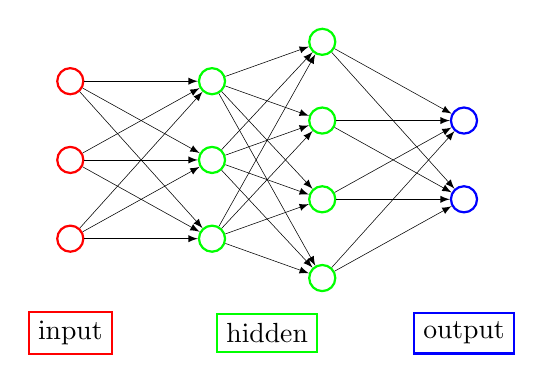
\begin{tikzpicture}
\usetikzlibrary{patterns}
\begin{scope}[very thin]
\foreach \x in {0, ..., 2} {
\node[circle, draw, color=red, thick] (input \x) at (-3, \x) {};
}
\foreach \x in {0, ..., 2} {
  \node[circle, draw, color=green, thick] (hidden1 \x) at (-1.2, \x) {};
  \foreach \y in {0,...,2}
    \draw[-latex] (input \y) -- (hidden1 \x);
}

\foreach \x in {0, ..., 3} {
  \node[circle, draw,color=green, thick] (hidden2 \x) at (0.2, \x-0.5) {};
  \foreach \y in {0, ..., 2}
    \draw[-latex] (hidden1 \y) -- (hidden2 \x);
}

\foreach \x in {0, ..., 1} {
  \node[circle, draw,color=blue, thick] (output \x) at (2, \x +0.5) {};
  \foreach \y in {0, ..., 3}
    \draw[-latex] (hidden2 \y) -- (output \x);
}

\node[rectangle, draw, color=red, text=black, thick] () at (-3, -1.2) {input};
\node[rectangle, draw, color=green, text=black, thick] () at (-.5, -1.2) {hidden};
\node[rectangle, draw, color=blue, text=black, thick]() at (2, -1.2) {output};
\end{scope}
\end{tikzpicture}
  }
  \caption{Architecture of nodes in a feedforward neural network. Each node receives the outputs of the previous layer.}\label{ann-layers} 
\end{figure}

A layer is a composed of \emph{nodes} (also called \emph{neurons}). A node accepts as input the previous layer's nodes' outputs, calculates a linear combination of them and applies a nonlinear function, called \emph{activation} function to the result (see~\ref{ann-nodes}). The typical choices for the activation function are sigmoid: $\frac{1}{1 + e^{-x}}$, hyperbolic tangent, and (popularized recently) rectified linear unit (ReLU): $\max(0, x)$.\footnote{A thorough, yet comprehensible discussion of the various activation functions can be found in~\cite{cs231-actfun}.}
\begin{figure}[h]
  \centering
  \resizebox{0.7\textwidth}{!}{
  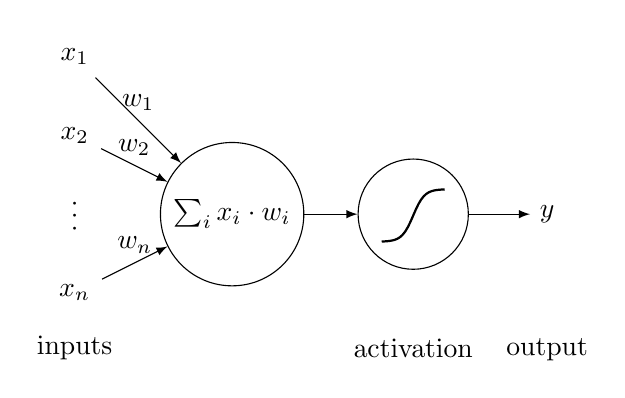
\begin{tikzpicture}[]
\node[circle](x1) at (-2, 2) {$x_1$};
\node[circle](x2) at (-2, 1) {$x_2$};

\node[circle](xn) at (-2, -1) {$x_n$};
\path (x2) -- node[rotate=90]{\ldots} (xn) ;
\node[circle, draw](center) at (0, 0) {$\sum_i x_i \cdot w_i$};
\node[circle, draw, minimum width=1.4cm](activ) at (2.3, 0) {};
\node (output) at (4, 0) {$y$};

\draw[domain=1.9:2.7, thick] plot (\x, {1/(1.5*(1+exp(-14*(\x-2.3)))) - .35});

%\draw[thick] (1.85 , -0.2) --  (2.5, -0.2) -- (2.8, 0.4);

\draw[-latex]  (center) -- (activ);
\draw[-latex] (x1) -- node[above]{$w_1$} (center);
\draw[-latex] (x2) -- node[above]{$w_2$}(center);
\draw[-latex] (xn) -- node[above]{$w_n$}(center);
\draw[-latex] (activ) -- (output);

\node ( ) at (-2,-1.7) {inputs};
\node ( ) at (2.3,-1.7) {activation};
\node ( ) at (4,-1.72) {output};

\end{tikzpicture}

}
  \caption{Details of a neural network node.} \label{ann-nodes}
\end{figure}

The trainable parameters of the model are weights of the linear combination of each of the nodes. The intuition behind introducing multilayer, multinode architecture is that different nodes will learn different statistics useful for producing the output, e.g.~eye or nose detectors for face recognition. The neurons from the earlier layers will learn simple dependencies in the data (e.g.~detection of edges) and the further neurons will combine their information, finding more sophisticated relations (e.g.~dog detector neurons).

\subsection{Gradient descent}\label{gradient descent}
There are a lot of optimization algorithms used to train neural networks, i.e.~find the best set of parameters (weights) for a given network architecture and the data. All of them are a modification of an algorithm of gradient descent \cite{gradient-descent}.

To use it, we first need to choose a loss function, which is a differentiable function of the output of the neural network that correlates with how well the model is doing its job; its value should be high for the bad models and low for the good  models. For example, if we want to predict the depth of each pixel in a photo (useful e.g.~for self-driving cars), we could use a dataset of images accompanied with their depths estimated with a 3D~camera. As a loss function, we could use a mean-squared~error between the real depths and those predicted by the model:
$$
L = \frac{1}{\mbox{\# images}}\sum_{image} \sum_{x, y} (\mbox{real\_depth}(image, x, y) - \mbox{model\_output}(image, x, y))^2
$$

Then, to update the weights of the model to minimize the loss, gradient descent calculates the gradient of the loss with respect to every parameter of the model and moves the weights in the direction of the steepest descent by a small amount~$\varepsilon$, called~\emph{step~size} or \emph{learning~rate}. Choice of a bigger $\varepsilon$ leads to faster learning, but makes the optimization prone to missing good areas of space or diverging completely. Smaller step~size leads to more stable
learning.

The gradients of every weight is determined with the help of chain rule:
\begin{equation}\label{chain rule}
  \frac{\partial}{\partial x} (f \circ g) = (\frac{\partial}{\partial x} f \circ g\big) \cdot \frac{\partial}{\partial x}g
\end{equation}
The equation~\eqref{chain rule} suggests an order of calculating the derivatives: we should first calculate the ones of the weights in the output layer, then previous hidden layer, and so on until the input layer. For example with squared error, sigmoid activation function, datapoints~$x_i$, and target outputs~$y_i$ we have:
\begin{multline}
  \frac{\partial L}{\partial w_{\text{input}, 1}} = \frac{\partial}{\partial w_{\text{input}, 1}} \sum_{i} (y_i - \text{output}(x_i))^2 =\\=  \sum_{i} 2(y_i - \text{output}(x_i)) * \frac{\partial}{\partial w_{\text{input}, 1}}
  ( y_i - \text{sigmoid}(\sum_j w_{\text{output}, j} \cdot \text{hidden}(x_i, j))) =\\=
  \underbrace{\sum_{i} -2(y_i - \text{output}(x_i)) * \text{sigmoid'}(\sum_j w_{\text{output}, j} \cdot \text{hidden}(x_i, j)) * \sum_j \text{hidden}(x_i, j)}_{\sum_j \frac{\partial L}{\partial w_{\text{output}, j}}} * \frac{\partial}{\partial w_{\text{input}, 1}}\ldots
\end{multline}

Because the process of gradient calculation proceeds from the end of the network toward the beginning, it is called \emph{backpropagation} or \emph{backward~pass} (in contrast to \emph{forward} pass, when the network is evaluating outputs).

The calculation of a full loss, based on all examples can be infeasible: current datasets often consist of tens of gigabytes of data (see e.g.~coco challenge dataset:~\cite{coco-dataset}) and to train a network it is often needed to make a couple of thousands of parameter updates.
To speed the process up, it is common to approximate the full loss function (thus the gradients, too) by a loss calculated on a random subset of data examples. More often than not, a random subset of $100$~examples will possess statistical properties indistinguishable from the whole dataset, leading to accurate (and fast to obtain) estimates of gradients. This process is called \emph{minibatch} training (and the whole algorithm a \emph{stochastic}~gradient~descent) and the size of the \emph{batch} is another hyperparameter of the model. There is a trade-off in its choice---bigger batch size gives better gradient estimates, but takes longer to calculate.

The role of nodes in a neural network is symmetric---there's no reason a particular neuron should behave differently than its neighbor. To enforce neurons to learn various aspects of the data, we initialize the weights randomly. The experiments show that it suffices to make different neurons learn different weights---intuitively, the model with different neurons will have easier time predicting output, as it will be combining various types of information.

One can summarize this section by presenting a stochastic gradient descent pseudocode in algorithm~\ref{sgd-pseudo}. An example implementation for a toy problem can be found in file \texttt{code/gradient-descent.ipynb} on the CD.

\begin{algorithm} \label{sgd-pseudo}
  initialize all weights randomly\;
  \While{\text{not converged \& not exceeded maximum number of iterations}} {
    pick a random subset $S$ of data examples\;
    calculate the loss function for the examples in $S$ in forward pass\;
    calculate the gradients of the loss and update each weight in a backward pass:
    $w := w - \varepsilon \cdot \frac{\partial L}{\partial w}$
  }
  \caption{Pseudocode of gradient descent.}
\end{algorithm}

\section{Deep Learning}
The neural networks were not often applied in modelling until recently. There was a number of factors which contributed to their current successes. In this section we describe shortly the most important of them.

\subsection{Computing power}
Creating top prediction or classification models requires a lot of computation power.\footnote{Deep learning community jokes that the time to train a state-of-the-art model stays a week, regardless of the increase in the computing power.} Neural networks, with their big expression power can provide good results, but only when supplied with enough data. When we pass a little data to a deep neural network, we can often see an \emph{overfitting} effect---the model performs well on the data it saw (training data), but generalizes poorly to unseen examples (test data).

In a world with limited computation power, best results will be biased towards simpler models, like linear regression, random forest, or support vector machines. Out of the whole continuum of~$R^n \rightarrow R^m$ functions, elementary models will pick a small subset of smooth, easy, reasonable ones and will pick the best one with the use of limited data. As the subset of functions that can be expressed is small, they are quite different from each other and it is easy for the model to pick the best function.

When a more involved model is trained, it can represent more functions, but at the expense that it requires more data (thus more computation power). When faced with data scarcity, it doesn't choose the best function among all that it can represent---it falsely detects noise in the data as significant patterns and erroneously treats insufficiently often occurring patterns as noise.

Fortunately, thanks to game industry, we saw a rapid increase in computation speed and memory bandwidth of graphics processing units (see figure~\ref{nvidia-speed}). These processors allow for executing matrix operations much faster than regular CPUs. Both forward and backward passes of a neural network can be expressed as few matrix operations, leading to efficient training of neural networks on GPU. In our experiments we saw more than ten-fold speedups moving from a high-end CPU to a middle range GPU.

\begin{figure}[h]
  \includegraphics[width=\linewidth]{images/gpu-bandwidth.png}
  \caption{Comparison of best CPU and GPU memory bandwidths in time. Note that the memory bandwidth often constraints the speed of neural network training. Plot comes from \cite{nvidia-docs}.}\label{nvidia-speed}
\end{figure}

\subsection{Vanishing and exploding gradients}
\optional{relu saturation}

\subsection{Better training algorithms}
The speed of convergence of vanilla stochastic gradient descent can be improved in many cases. For example, if the optimization space is a valley with high hills and a river with a little slope in the bottom, SGD will zigzag from one wall of the valley to the other, due to higher gradients between the walls than in the river. \optional{picture}

There are a lot of improvements of the SGD to faster move in the optimization space in the situations like this. They include momentum~\cite{momentum}, Adam~\cite{adam}, or Adadelta~\cite{adadelta}. I will describe RMSProp~\cite{rmsprop}, the algorithm that we use in our code. One can read about the others in~\cite[chapter 8.3.]{dlbook} in detail.

\subsubsection{RMSProp}\label{rmsprop-section}
The basic idea of RMSProp is dividing the gradient by the square root of the sum of previous gradients' squares pointwise. This way the directions which keep having high gradients in the course of training, will be scaled more and more and directions will low gradients will be more and more ``preferred'' to traverse along.

To prevent vanishing the learning rate too much and significantly slowing down the learning near the end, instead of calculating the sum, RMSProp stores the exponential average of the history of gradients' squares.

The pseudocode of RMSProp can be found in algorithm~\ref{rmsprop-pseudo}.
\begin{algorithm}
  \DontPrintSemicolon
  \SetKwInOut{Input}{input}
  \Input{Initial parameters $\theta$, learning rate $\varepsilon$, decay rate $\rho$, small constant $\delta$ for numerical stability}
  Initialize gradient accumulation $r \leftarrow 0$\;
  \While{not converged}{
    Pick a random subset $S$ of data examples\;
    Calculate gradient: $g \leftarrow \nabla_\theta \sum_{(x, y)\in S} L(f(x, \theta), y)$\;
    Accumulate squared gradient: $r \leftarrow \rho r + (1-\rho) g \cdot g$ (pointwise multiplication)\;
    Compute parameter update: $\Delta\theta \leftarrow \frac{-\varepsilon}{\sqrt{\delta + r}} \cdot g$ (pointwise multiplication)\;
    Update parameters: $\theta \leftarrow \theta + \Delta \theta$\;
  }
  \caption{Pseudocode of RMSProp, adapted from~\cite{dlbook}.}\label{rmsprop-pseudo}
\end{algorithm}

\subsection{Convenient libraries}
Another factor causing deep learning models to rise is the creation of open source libraries for symbolic computation. A mere $6$~years~ago, if a student or a scientist wanted to experiment with neural network models, he had to implement the neural network as a couple of matrix multiplications, calculate the gradients on paper and backpropagate them in code, and implement a version of gradient descent. Not to mention that performing the computation on GPU using a direct memory manipulation like CUDA increased the code complexity twice.

Fortunately, around~$2010$ open source libraries, greatly simplifying the process of implementing deep learning models, started to appear. Currently there are $3$~such frameworks which are popular: Theano, Torch and Tensorflow.

Theano~\cite{theano} is a python library developed by Montreal Institute for Learning Algorithms, which the author made a humble contribution to.\footnote{The contribution can be accessed in~\cite{theano-contrib} and contains possibility of evaluation just a subset of outputs of an already compiled theano function.}

Torch~\cite{torch} is a library allowing to write neural networks in Lua, used and developed by Facebook.

Tensorflow~\cite{tensorflow} is a library made by Google, supporting writing in C\texttt{++} and python. It was the first to seamlessly allow the distributed training of models.

The ideas behind these libraries are similar. All of them allow the user to write the high-level code that will be interpreted as a symbolic computation forming a directed acyclic graph. Then, during execution, it is compiled to a low-level code able to run on a GPU. The libraries decide on the order of calculating the nodes in the graph (called~\emph{Op}s).

Treating the code written by the user as symbolic expressions and deferring its evaluation allow to perform low-level optimization (like in compilers---in a sense these libraries \textit{are} compilers), symbolically calculate the gradient of an expression, and allow for different backends (CPU~vs.~GPU).

\renewcommand{\figurename}{Snippet}
You can see a short example of Theano code in snippet~\ref{theano-code}, which is also available as \texttt{code/theano.ipynb} on the CD.

\begin{figure}[!h]
\begin{Verbatim}[commandchars=\\\{\}]
{\color{incolor}In [{\color{incolor}1}]:} \PY{k+kn}{import} \PY{n+nn}{theano}
        
        \PY{n}{x} \PY{o}{=} \PY{n}{theano}\PY{o}{.}\PY{n}{tensor}\PY{o}{.}\PY{n}{dscalar}\PY{p}{(}\PY{l+s+s2}{\PYZdq{}}\PY{l+s+s2}{x}\PY{l+s+s2}{\PYZdq{}}\PY{p}{)}
        \PY{n}{y} \PY{o}{=} \PY{l+m+mi}{3} \PY{o}{*} \PY{n}{x} \PY{o}{\PYZhy{}} \PY{n}{x} \PY{o}{*} \PY{n}{x}
        \PY{n}{dy} \PY{o}{=} \PY{n}{theano}\PY{o}{.}\PY{n}{tensor}\PY{o}{.}\PY{n}{grad}\PY{p}{(}\PY{n}{y}\PY{p}{,} \PY{p}{[}\PY{n}{x}\PY{p}{]}\PY{p}{)}\PY{p}{[}\PY{l+m+mi}{0}\PY{p}{]} \PY{c+c1}{\PYZsh{} \PYZhy{}2x + 3}
        \PY{n}{f} \PY{o}{=} \PY{n}{theano}\PY{o}{.}\PY{n}{function}\PY{p}{(}\PY{n}{inputs}\PY{o}{=}\PY{p}{[}\PY{n}{x}\PY{p}{]}\PY{p}{,} \PY{n}{outputs}\PY{o}{=}\PY{p}{[}\PY{n}{y}\PY{p}{,} \PY{n}{dy}\PY{p}{]}\PY{p}{)}
        \PY{n}{f}\PY{p}{(}\PY{l+m+mi}{3}\PY{p}{)}
\end{Verbatim}

            \begin{Verbatim}[commandchars=\\\{\}]
{\color{outcolor}Out[{\color{outcolor}1}]:} [array(0.0), array(-3.0)]
\end{Verbatim}
              \cprotect\caption{Example Theano code}
              \label{theano-code}
\end{figure}

\renewcommand{\figurename}{Figure}
Theano, Torch and Tensorflow in their basic form are libraries to express any kind of computation. The popularization of them fueled the creation of many higher level frameworks, even further simplifying implementation of deep models. These libraries, including Keras~\cite{keras}, blocks~\cite{blocks} and TFLearn~\cite{tflearn} allow for implementing typical transformations, like an all connected layer, softmax, or popular activation functions, in one line. They make it easier to read the data, visualize the learning process, and implement the popular optimization algorithms.

\section{Atari~2600}
Atari~2600~\cite{atari} is a game console created in the late 70s. It has a processor running at around~$1$~MHz, mere $128$~bytes of RAM~memory and a joystick with $18$~actions ($9$~positions $\times \{\mbox{fire}, \mbox{no-fire}\}$). To play a game, one needs to insert a cartridge with a ROM of a game (of size $4kB$) and connect the console to the TV~screen. It was producing a new game screen with frequency~$60Hz$ using some tricks,\footnote{Interested reader can read a short article about ``racing the beam'' in~\cite{racing-beam}.} needed to show the full image when the RAM fitted only a line of it. A picture of the Atari~2600 can be seen in figure~\ref{atari-picture}.

\begin{figure}
  \centering
  \includegraphics[width=.8\linewidth]{images/atari.jpg}
  \caption{Picture of the Atari machine.}\label{atari-picture}
\end{figure}

The interest in Atari within AI community arose after the publication of~\cite{ale}. It introduces Arcade Learning Environment, a framework which allows for easy creation and evaluation of agents playing Atari games. It encompasses Stella~\cite{stella}, the Atari~simulator for computers. Thanks to~ALE, the programmer can read the screen as a python array, know which actions are possible in each game and read rewards without the need to parse them from the screen nor understanding the details of RAM~memory of each game.

Some time after the release of~ALE, OpenAI, an emerging player in AI, created a convenient wrapper on top of it: OpenAI~Gym~\cite{gym}. It further simplifies the evaluation of the agents, introduces some new, non-Atari environments to test the agents, and make it possible to visualize the training on OpenAI~page, encouraging scientists to open source their ideas.

The diversity of Atari games made it a good challenge for AI agents. There are both very simple games, like Pong, where a good initial position of the paddle can guarantee winning and very involved ones, like Montezuma's~Revenge requiring to collect items and use them correctly.\footnote{The best to our knowledge method for Montezuma's~Revenge~\cite{hdqn}, requires manual formulation of the game's objects and sub-goals, what makes it hardly transferable to other environments.} The work on creating agents capable to play many of the Atari games well resulted in many breakthroughs in AI, including winning the Go game with a human world-champion~\cite{alphago} and creation of deep~Q-learning, to which the next chapter is dedicated.


\chapter{Deep Q-learning}\label{dqn}
Deep Q-learning\footnote{known also as deep Q networks or DQN} is a reinforcement learning algorithm introduced in~\cite{nips-dqn}. It is known for being able to learn agents to play Atari games using the game screen as input. Mathematically, it is an extension of Q-learning (described in section~\ref{qlearning}), using neural networks as a Q-value approximator.

Even though Q-learning is a correct algorithm in a sense that it converges in the limit to the optimal strategy, the rate of this convergence is slow. It comes to no surprise---to propagate the rewards and correctly estimate Q-values of all states, each of them have to be visited multiple times.\footnote{\cite{qlearning-complexity} presents theoretical analysis of Q-learning speed of convergence. The raw Q-learning's complexity is estimated as $O(n^3)$ in the number of states.}
With raw Atari frames of size~$210 \times 160 \times 3$ (width $\times$ height $\times \{\text{R}, \text{G}, \text{B}\}$) and color depth of~$128$, the number of possible input states can be estimated as:
\begin{equation}
  \mbox{\# states} = 128^{210*160*3} \approx (2^7)^{2^{16}} \approx 2^{2^{18}} \approx 2^{256000}
\end{equation}\label{number-frame-states}
which is way to much to store in this universe, not to mention process multiple times on a computer.

Main idea of deep Q-learning is to use some form of generalization between states. This way, seeing a reward in a given state-action pair, we will get information not only about this particular state, but about similar states as well. This will also let us to store the Q-value function in a concise form, alleviating the exponential state explosion problem outlined above.

To model a problem with a neural network, we have to define a differential loss function to minimize (compare section~\ref{gradient descent}). In the case of deep Q-learning, a natural choice is some function of the difference between left- and right-hand sides of equation~\eqref{qlearning-property} (we know that the optimal strategies have this difference equal to~$0$), so a mean of squares of these differences was choosen:
\begin{equation}\label{dqn-loss}
  L(\theta_t) = \mathbb{E}_{s_t, a_t, s_{t+1}} \big(r_t + \gamma \max_b Q(s_{t+1}, b|\theta_{t-1}) - Q(s_t, a_t|\theta_t)\big)^2
\end{equation}
\todo{Put it as a definition and underline that $t$ comes from the context; say that we want to approximate it. Is there a theorem about the learning process with $L(\Theta_t)$? Maybe add that optimal strategies have this loss $0$.}
Let's explain notation in more detail. $Q$ is the function mapping state-action pairs to the estimation of their value (expected discounted reward). In our case the role of~$Q$ will be fulfilled by a neural network. The part~$|\theta_t$ comes from the fact that the values of~$Q$ function will be dependent on the current parameters $\theta_t$ of the network. $t$~is the discrete time in the episode. We define loss with regard to the parameters in time~$t$ ($L(\theta_t)$) using the current parameters~$\theta_{t-1}$---we want to be able to estimate ``goodness'' of any new parameters~($\theta_t$) based on~$\theta_{t-1}$. The estimation~sign~$\mathbb{E}_{s_t, a_t}$ comes from the fact we will not score all the state-action~pairs, but rather the ones that appear in real games. In fact, a more appropriate notation would be to sum over all the observed state-action~pairs; the current one is used to simplify notation.

We can differentiate the loss function with respect to the parameters:
\begin{multline}
  \nabla_{\theta_t} L(\theta_t) = \nabla_{\theta t}\, \mathbb{E}_{s_t, a_t, s_{t+1}} \big(r_t + \gamma \max_b Q(s_{t+1}, b|\theta_{t-1}) - Q(s_t, a_t|\theta_t)\big)^2
 =\\=
  \mathbb{E}_{s_t, a_t, s_{t+1}} \nabla_{\theta t} \big(r_t + \gamma \max_b Q(s_{t+1}, b|\theta_{t-1}) - Q(s_t, a_t|\theta_t)\big)^2
  =\\=
  \mathbb{E}_{a_t,s_t, s_{t+1}} 2\Big(
  r_t + \gamma \max_b Q(s_{t+1}, b|\theta_{t-1}) - Q(s_t, a_t|\theta_t)\Big)
  \nabla_{\theta_t} Q(s_t, a_t|\theta_t)
\end{multline}

Note that $\theta_{t-1}$ is treated as a constant with respect to~$\theta_t$. Even though this derivation is unnecessary to implement deep Q-learning (as it is usually done by a library), it gives some intuition about how our optimization algorithm will work.

$Q(s, a|\theta)$ will be implemented as a neural network that accepts the state of the game and returns a multidimensional vector---each coordinate will correspond to a Q-value of one action. At each time step, we will query the network with current state and make the action with the highest Q-value.
Then, we will collect tuples:~$s_t, a_t, r_t, s_{t+1}$ of current state, performed action, received (immediate) reward and the next state. To use such a tuple to decrease the loss~\eqref{dqn-loss}, we will calculate $\max_b Q(s_{t+1}, b)$ and~$Q(s_t, a)$ in a forward pass through the network, and $\nabla_{\theta_t} Q(s_t, a_t)$ using backpropagation (starting from the output node corresponding to the chosen action). We will use these expressions to calculate the derivative of the loss~$\nabla_{\theta_t} L(\theta_t)$ and update the parameters using RMSProp---a modification of gradient~descent described in section~\ref{rmsprop-section}.

The core algorithm, defined above, is not powerful enough to learn to successfully play Atari games using screen output. To make it work better, authors employed a couple of improvements, described below.

\section{Preprocessing the screen}
Low-detail graphics of Atari games have low information~density. If we entered the screens as they was to the network, it would have to learn the dependencies between pixels itself, leading to less stable and longer training. To circumvent this problem, authors of DQN downscale the screens to gray-scale~$110 \times 84$ images. Then, they further crop the central square of~$84 \times 84$ pixels of the image, to be able to easily pass it as input to a convolutional network.\footnote{Convolutional networks, as more appropriate to process screen than the main topic of this work---RAM, are not described in detail here. A detailed explanation of convnets can be found in chapter~9 of~\cite{dlbook}.}

\section{Exploration-exploitation trade-off}
When we play the game using Q-learning, we choose the actions that have the highest Q-values for the state we are in. For testing, that is a reasonable approach---we want our agent to play as good as he could, given current state value~estimation. But for training, the following scenario can happen: during our first game, say we chose action~$a_0$ in the initial state~$s_0$, proceeding to~$s_1$. We received some small, but non-zero reward~$r$ and continued the game from there. When we started the second game, we were obliged to use the action~$a_0$ in~$s_0$, as it is associated with non-zero reward (and we have little knowledge about the state value anyway). We will be doing this choice on and on, until the value estimation of state~$s_1$ drop, so that the small reward will be outweighed by it.

In this situation, our basically random choice at the start of training influences our behavior for a very long time, preventing us from trying other options, that may be more viable. This problem is known as exploration-exploitation trade-off; on one hand, we would like to make the best actions we know (to $\emph{exploit}$), but on the other, we would like to build our knowledge about the effects of different actions (to $\emph{explore}$).

One of the solution to this problem, is, instead of using a greedy strategy (choosing the actions with the best Q-values), to use so called $\varepsilon$-greedy~strategy---to choose a random action with probability~$\varepsilon$, and with probability~$1 - \varepsilon$ the one with the highest Q-value estimation. By choosing~$\varepsilon$ we decide how much time we want our agent to spend on exploring new actions vs. exploiting the ones he knows are good.

This technique is not uniquely associated with DQN; in fact it was used with bare Q-learning and other reinforcement learning algorithms from early on.

\discussed

\subsection{$\varepsilon$~decay}
To set the exploration-exploitation trade-off in an appropriate place, the DQN inventors decided to use changing~$\varepsilon$, namely one decaying linearly from~$1$ to~$0.1$. This way, at the beginning of training, when the state value estimations are poor, the agent does more exploration of new actions and further in the game, he chooses the best action according to the Q-values of states more often. Note that the random actions are done only in the training part---when the performance of a trained agent is evaluated, a flat, low value of $\varepsilon=0.05$ is used.

\section{Frameskip}\label{dqn-frameskip}
In many Atari games, developers use visual illusion to make games look better. For example, in Space Invaders, in which the aim of the user is to shoot down the enemy ships and avoid their shots, the shots are not shown on the screen on every frame. Instead, the user can see the shot on one frame, then for a couple of frames the shot cannot be seen on the screen, then it appears somewhere further. For humans, the illusion of movement is good enough.

If we tried to pass the one-frame input to the neural network, it'll have problems learning the appropriate Q-values, because without seeing the shot, the network will not know if in the next state the player will be hit and will lose a life or the enemy will be killed and user will gain points. Formally speaking, the markovian assumption we were using from the very beginning will be violated.

The solution to this problem is to pass not the last frame of the game, but the last $k$~frames (in~\cite{nips-dqn}, $k=4$ is used for most of the games) to the network, choose the action based on those frames and repeat it $k$~times.

This serves two purposes. First, it solves the problem of ``blinking'' objects, unless they disappear for at least $k$~frames.

Second, it helps for learning dynamics of the model. Let's imagine the agent is in a state, such that he will receive a big reward if he presses ``left'' for half a second. Assuming $A$~possible actions, $60$~frames per second, and basically random actions at the beginning, this will happen with probability~$A^{-(60 / 2)}$. If we change the action every $k=4$~frames, the probability to make the left movement for half a second will dramatically increase to~$A^{-(60/(4 \cdot 2))}$, as we will now make $4$~times less decisions.

Of course, this improvement (called frameskip) limits the amount of strategies that we can learn---our agents are now only able to express strategies that change actions at least every $k$~frames, but, unless the game need superhuman reflex (like, e.g.,~boxing~\cite{boxing}), using bigger than~$1$ frameskip value helps to train better agents in practice.

\section{Experience replay}\label{experience-replay}
Another method used to effectively train the neural network agents used in DQN is experience replay. Training a neural network to achieve good performance can be a long process. For a regular supervised tasks, like image recognition or machine translation is it not uncommon to have to process the whole dataset multiple (tens to hundreds) of times (called epochs) to get the optimal parameters for given hyperparameters, even with the use of minibatch training.

In the reinforcement learning setting, we don't have a dataset per se, we rather interact with environment and observe its reactions. To be able to reuse the training examples multiple times, we save the history of our interactions with environment (in a form of a list of tuples, containing $($state,~action,~reward,~next~state$)$) in the memory. During training, we do the actions according to the strategy defined by the network's Q-values estimation, but to update the weights, we choose a random batch of tuples from the memory and calculate the gradients using them.

This method allows us to look at each interaction (example) multiple times during training. It also improves statistical properties of the gradient: as we use stochastic gradient descent, we would like examples in each batch to be representative of the whole history of observations; choosing the elements of the batch randomly, we achieve better estimate of the full loss, as the consecutive observations are strongly correlated.

Due to the limits in the size of memory, the history of interactions contain last $n$ (in the order of tens-hundred to millions), not all past observations.


\chapter{Deep Q-learning for RAM}
Here we describe our contribution -- the network architectures, etc.

\section{Tricks}
\subsection{Dropout}
\subsection{Frameskip}
\subsection{Joining RAM and screen}
\subsection{Learning rate}
\subsection{Unrolling frameskip}
\subsection{RNN}


\chapter{Results}
\todo{Describe the evaluation procedure}
\todo{Describe the games we were evaluating on}
\todo{Tell that we didn't test on all of the games, because computing power}
\todo{Tell how long it took to train one game}
\todo{Show the numerical results we got with a plain approach}
\todo{Show the numerical results we got with dropout}
\todo{Show the numerical results for frameskip}
\todo{Show the numerical results for learning rate}
\todo{Show the numerical results for joining RAM+image}

\todo{Show the visualization of the first layers}


\chapter{Future work}
Interesting ideas for continuing this line of research.



\begin{appendices}
  
\chapter{ICM cluster setup}\label{icm}
Most of the experiments we executed during the project were ran on a cluster of Interdisciplinary Centre for Mathematical and Computational Modelling of University of Warsaw (known as ICM). We got a lot of experience using these machines and decided to write it up in this appendix in the hope that it may be a useful guide for someone else doing a deep learning project using the ICM's architecture.

\section{Hardware architecture}
  ICM owns a couple of computing clusters for different purposes. We used the only one containing GPU cards: Grom~\cite[in polish]{grom-icm}. It contains an ssh server and a number of computational nodes. You can ssh to the ssh server only, and from there you can insert a job into a Slurm~\cite{slurm} queue. A job can be an interactive bash session, which is very convenient to try things out.
  
  The specification of the job uses Slurm format, but the commands to execute can be any bash commands. One flag worth to mention is \texttt{-{}-gres}, which allows to specify request for GPU. You can see an example Slurm job specification in listing~\ref{slurm-file}.

  \begin{lstlisting}[language=bash, caption={Example Slurm job specification}, label={slurm-file}]
#!/bin/bash -l
#SBATCH -J dqn
#SBATCH -N 1
#SBATCH --ntasks-per-node 8
#SBATCH --mem 4000
#SBATCH --time=165:00:00
#SBATCH --gres=gpu:1
#SBTACH --output="logs"
#SBATCH --exclude wn8002,wn8006
#SBATCH -C cuda

source /icm/home/sygnowsk/dqn/deep_q_rl/venv/bin/activate
python run_sygi.py -r enduro.bin --network-type big_ram
\end{lstlisting}

The job will be executed on one\footnote{It is possible to reserve more nodes for one job, but we didn't use that feature.} of the $24$~computational nodes, each having $2$~NVIDIA~GTX~$480$ cards. During our experiments, to fully utilize the resources, we limited the memory and GPU number requirements to be able to run two experiments in each node in parallel.

\section{Software stack}
  The operating system installed on the Grom cluster is CentOS6. The main system is quite raw, and to make use of it, one needs to use modules (loaded using command \texttt{module load NAME}) with compilers, libraries, etc.

  During the first try to run DQN we wanted to use the code provided by the authors of the algorithm, which was written using Torch. Even though Lua, as well as its package manager luarocks was installed in the system, we were having hard time installing the code dependencies without root privileges.

  Due to these problems, we decided to move to code based on Theano, which is based on python. We downloaded a standalone python script enabling \texttt{virtualenv}, which allows to encapsulate a project's python dependencies in a local directory, making it possible to install python libraries locally. The only library we had to install from sources was OpenCV, whose python version: \texttt{opencv2} is just a wrapper around the regular OpenCV and expects the library to be already installed in the system.

\section{Running experiments}
  The result of running the experiment was a directory with a file listing the results of training after each epoch and one file per epoch with the network parameters, as well as a Slurm file with output from stdout and stderr. The parameters were serialized using python package \texttt{pickle}.

  As one job usually took a day or two to finish, it was often the case that there was a number of jobs in progress and it was hard to distinguish, which was which. To tackle this problem we updated the code to output not only evaluation results, but also all the hyperparameters of the model.

  After we finished our experiments, a company deepsense.io released a tool: Neptune, which aims to simplify management of experiments.

\chapter{Hyperparameters}\label{hyperparams}
The list of hyperparameters and their descriptions. Most of the descriptions come from \cite{nature-dqn}.
\begin{table}[h]
\begin{tabularx}{\textwidth}{@{} l c Y @{}}
\toprule
hyperparameter & value & description \\
\midrule
minibatch size & $32$ & Number of training cases over which each stochastic gradient descent (SGD) update is computed. \\\addlinespace
replay memory size & $100\,000$ & SGD updates are randomply sampled from this number of most recent frames. \\\addlinespace
phi length & $4$ & The number of most recent frames experienced by the agent that are given as input to the Q network in case of the networks that accept screen as input. \\\addlinespace
update rule & \texttt{rmsprop} &  Name of the algorithm optimizing the neural network's objective function   \\ \addlinespace
learning rate &  $0.0002$  & The learning rate for rmsprop\\ \addlinespace
discount & $0.95$ & Discount factor $\gamma$ used in the Q-learning update. Measures how much less do we value our expectation of the value of the state in comparison to observed reward.\\\addlinespace
epsilon start & $1.0$ & The probability ($\varepsilon$) of choosing a random action at the beginning of the training. \\\addlinespace
epsilon decay & $1000000$ & Number of frames over which the $\varepsilon$ is faded out to its final value. \\\addlinespace
epsilon min & $0.1$ & The final value of $\varepsilon$, the probability of choosing a random action. \\\addlinespace
replay start size & $100$ & The number of frames the learner does just the random actions to populate the replay memory.\\
\bottomrule
\end{tabularx}
\caption{Hyperparameters used by our models.}
\label{table:param}
\end{table}

\end{appendices}


\cleardoublepage
\phantomsection % to make sure the page number for Bibliograhpy is correct

\addcontentsline{toc}{chapter}{Bibliography}
\printbibliography

\end{document}
